\chapter{Introduction}\label{ch:introduction}

\section{Motivation and Problem Statement}\label{sec:motivation}

Interpretability is moving from a tool for inspecting model decisions post hoc to a practical mechanism for improving and controlling models. Interpretations increasingly guide model correction, training, and inference~\parencite{Anders2020ClArC,Pahde2023R2R,Ross2017RightReasons,Komorowski2026AGD}.
Attribution can help identify internal components for testing or intervention, and can guide model correction or inference. Errors in such explanations can affect the resulting intervention. We therefore ask what these explanations explain about the computation of a trained network.

Three research questions organize this account. \emph{What structure can be exposed without changing the network's function?} \emph{What does a backward attribution actually calculate?} \emph{How can these representations guide the design and evaluation of attribution methods for visual inspection?}

For vision models, this question concerns a form of shared visual grounding. When we ask a machine what it sees, seek its help, or entrust it with a task, we expect some alignment between its use of visual information and our own understanding of the scene. A robot asked to grasp a cup should recognize its shape and position. A system assisting a radiologist should attend to signs of disease, rather than incidental clues about where the image was acquired---a shortcut documented in medical imaging~\parencite{Zech2018Pneumonia}. We therefore seek models whose decisions rest on task-relevant objects, features, and relations in a way we can understand and question. Attribution offers a means of investigating this alignment, providing evidence for communication, justified trust, and correction.

Heatmaps make this question concrete: is a prediction supported by relevant features, or by an incidental artifact? Attribution has exposed such ``Clever Hans'' strategies~\parencite{Lapuschkin2019}, which can undermine generalization when familiar correlations change~\parencite{Geirhos2020Shortcut}. In vision systems that guide physical actions, these failures pose safety concerns. Deliberate visual manipulations also create security risks, as physical attacks on road-sign classifiers demonstrate~\parencite{Eykholt2018Physical}. Heatmaps can identify suspicious dependencies for further testing, although visual inspection alone does not establish robustness or safety. Attribution is also used to investigate spurious behavior in anomaly detection and explain one-class models~\parencite{Kauffmann2020CleverHans,Kauffmann2018OneClassDTD}.

This thesis focuses on white-box, backpropagation-based attribution methods, which use a network's weights, activations, and computational graph. Black-box methods such as LIME and KernelSHAP instead query the model's input--output behavior~\parencite{Ribeiro2016,LundbergLee2017}. Access to the network's internal computation allows us to ask how an attribution arises from its learned weights and activations, and what its propagation rule measures. Beyond the input--output dependencies examined by black-box methods, this access may help locate unwanted dependencies within the network, providing a promising direction for targeted model correction and training.
Internal access provides targets for correction in hidden representations and allows explanation-based penalties to enter the training objective. Constraints on input gradients can penalize sensitivity to annotated irrelevant inputs~\parencite{Ross2017RightReasons} or encourage adversarial robustness~\parencite{Ross2018InputGradients}; Projective Class Artifact Compensation (P-ClArC) suppresses identified artifact directions in intermediate activations~\parencite{Anders2020ClArC}, while Reveal to Revise combines detection and correction in an iterative model-development cycle~\parencite{Pahde2023R2R}. Mechanistic Shaping extends this approach by using attribution penalties on internal concept directions to discourage unwanted reliance during training, including reliance on spurious backgrounds in vision models~\parencite{Fel2026MechanisticShaping}.

Interpretability increasingly studies concepts and internal features alongside input heatmaps. Concept Relevance Propagation (CRP) uses concept-conditioned LRP to connect predictions to learned concepts and their input evidence~\parencite{Achtibat2023CRP}. SemanticLens gives model components semantic descriptions and uses attribution to assess their contributions to predictions~\parencite{Dreyer2025SemanticLens}. Sparse autoencoders and related transcoders seek interpretable features; circuit tracing connects such features through attribution graphs of a local replacement model~\parencite{Ameisen2025CircuitTracing}. Across these approaches, attribution helps investigate how internal features contribute to a decision. Understanding its backward rules therefore remains relevant as explanations move from pixels to concepts.

Language models raise a further oversight problem: a model may conceal an objective or recognize that it is being evaluated without saying so. For example, a gradient-based readout of internal representations has surfaced signals of an implanted objective even on ordinary prompts~\parencite{Gurnee2026Workspace}; a follow-up found that replacing gradient transport with LRP rules can recover intermediate variables more reliably in early layers~\parencite{Blank2026RLens}. These examples make the backward rule consequential beyond vision and motivate our mathematical study of LRP on Transformers.

The reliability of that evidence cannot be taken for granted. Randomization sanity checks show that some attribution methods produce similar maps even after learned model parameters have been randomized~\parencite{Adebayo2018sanity}. An apparently informative heatmap may therefore reflect input structure or architectural properties more than the particular computation learned during training. Input dependence, perturbation fragility, and misleading modified-gradient structure raise related concerns~\parencite{Kindermans2018PatternAttribution,Ghorbani2019fragile,Nie2018guided,sixt2020whenexplanationslie}. These findings motivate a shift in the object of scrutiny: beyond asking what an attribution map looks like, we must understand the calculation producing it and how that calculation relates to the trained network.

Evaluation requires a precise account of what the metrics measure. \textcite{Lipton2018Mythos} distinguishes the different objectives often grouped under interpretability, and \textcite{DoshiVelezKim2017} argue that evaluation must match the intended application and audience. \textcite{Murdoch2019Interpretability} separate predictive accuracy, descriptive accuracy, and relevance to the user. Here, the immediate objects of study are the computation of a trained network and the backward rules used to attribute its output. We use Quantus~\parencite{Hedstrom2023} to select metrics of faithfulness, localization, and robustness, complemented by numerical-stability and parameter-randomization checks; a convincing heatmap alone does not establish that a model relies on the intended evidence.

A structural starting point is the opposition already present in the network's arithmetic. Signed weights combine reinforcing and opposing contributions into a single pre-activation, and activation gates determine what is passed onward. The resulting activation records their balance without separately displaying how those contributions accumulated. This suggests a \emph{debate} perspective: which contributions support a class score, which oppose it, and how does their interaction determine the result? The same distinction is already built into the $\alpha\beta$ rule of \ac{lrp}, which separates positive and negative contributions to a neuron's pre-activation, normalizes them separately, and weights their backward redistribution through $\alpha$ and $\beta$~\parencite{Bach2015}. Separating support and opposition thus connects two questions: how the network forms its output, and how an attribution method traces that output backward.

The central aim of this thesis is to develop a unified mathematical framework that connects the decomposition of trained network computations to the backward attribution methods applied to them. By exposing opposing contributions in structured representations and characterizing backward attribution through games on the computational graph, we seek to develop mathematical models that make explicit what information an attribution retains, how it propagates that information, and how its rules can be compared and systematically modified.

The first obstacle concerns the \emph{representation} being interpreted. Monotonicity has long provided useful structure for this problem~\parencite{Sill1997_MonotonicNetworks,Amos2017}: with non-negative weights and monotone activations, increasing an input cannot decrease the downstream response. Non-negative representations allow contributions to accumulate without cancellation between positive and negative weighted terms within a stream~\parencite{ayinde2018nonnegativity,lee1999nmf}. Monotonicity constraints can also express domain-specific fairness requirements~\parencite{Wang2020ShapeFairness}; they encode the chosen requirement rather than guarantee fairness on their own. For decisions such as medical treatment or parole, \textcite{rudin2019stop} argues for inherently interpretable models whose reasoning can be inspected directly. For an already trained, unconstrained network, however, changing its weights to impose monotonicity generally changes its predictions.

The \ac{dc} decomposition offers a different approach: instead of requiring the whole network to be monotone or convex, we express pretrained neural networks as a difference $f=g-h$ of two \emph{split-streams}. We call $(g,h)$ the \emph{split-pair} and the network implementing this representation the \emph{split network}. Constructed layer by layer from the trained weights, the split-streams are convex and monotone with respect to the paired input coordinates, while their difference recovers the original network~\parencite{hiddenMono}. This gives the debate perspective a concrete realization: one split-stream enters the class score positively, the other negatively, and their balance determines the output. They are not merely the positive and negative parts of the final score; they expose contributions throughout the computation.

Making this representation usable at depth is a substantive computational problem. The two split-streams can grow rapidly while their difference remains moderate, leading to severe floating-point cancellation. \emph{Hidden Monotonicity} develops stabilization of the forward and backward passes through the split network~\parencite{hiddenMono}.

To investigate the mechanisms of opposing split-streams exposed by DC decomposition of pretrained models, the MNIST difference-model experiments in Section~\ref{sec:dcinns} train two convex or monotone networks jointly. When the $h$-stream receives the complemented input $\mathbf{1}-x$, the displayed gradients show class-dependent sensitivities on present strokes and candidate missing-stroke locations (Figure~\ref{fig:mnist_split_ic_saliency}). These patterns give the debate perspective a visual counterpart and motivate a factual/counterfactual interpretation.

The second obstacle is the zoo of backward attribution rules: gradients as local sensitivities, \ac{lrp} as redistribution, Deep Taylor as local decomposition, and Transformer-specific extensions~\parencite{playingBackward2026}. We unify gradients and the full $\alpha\beta$-\ac{lrp} family through a common game-theoretic representation of backward attribution.
\textcite{Gaubert2025} prove that a ReLU network's forward output is the game value of a two-player Stopping Game on its graph: layers are rounds, neurons are states, input values are terminal payoffs, and the scalar output $f(x)$ is the game value. In \emph{Playing the Network Backward}~\parencite{playingBackward2026}, we reinterpret backward attribution as a distribution of weighted game trajectories through the network (Figure~\ref{fig:game_trajectory_overview}), yielding a framework to compare different backward attribution methods. We adapt the game to a novel Stopping Decomposition, separating paths with positive and negative contributions to the prediction (Lemma~\ref{lem:parity_path})---information that the original game formulation averages out. In this framework, propagation rules become equilibrium policies, and attribution maps are recovered from the discounted occupation measure of the induced trajectory distribution---an integral over the path distribution assigning relevance to each game state. We introduce two games: the Stopping Game (\acs{sg}), whose occupation measures recover the Jacobian (Theorem~\ref{thm:gradient_occupation}), and the entropy-regularized Routing Game (\acs{rg}) at temperature $\tau$, whose occupation measures recover the full $\alpha\beta$-\ac{lrp} family at its anchor $\tau=1$ (Theorem~\ref{thm:lrp_recovery}) on ReLU networks under the stated propagation conventions. For attention blocks, an oracle player whose best response recovers the QK-softmax supplies a fixed reference policy that guides the players' Value routing. With this reference, the game recovers the composite $\alpha\beta$ rule of the conditioned attention--Value map (Theorem~\ref{thm:attention_ab_recovery}), which extends the framework to attention modules; the same entropy regularization extends \ac{sg} from ReLU to Softplus networks. The debate idea therefore becomes more than a metaphor: the separation already used by $\alpha\beta$-\ac{lrp} is embedded in a two-player framework whose backward calculations can be compared with those of gradients (Figure~\ref{fig:game_trajectory_overview}).

\begin{figure}[t]
    \centering
    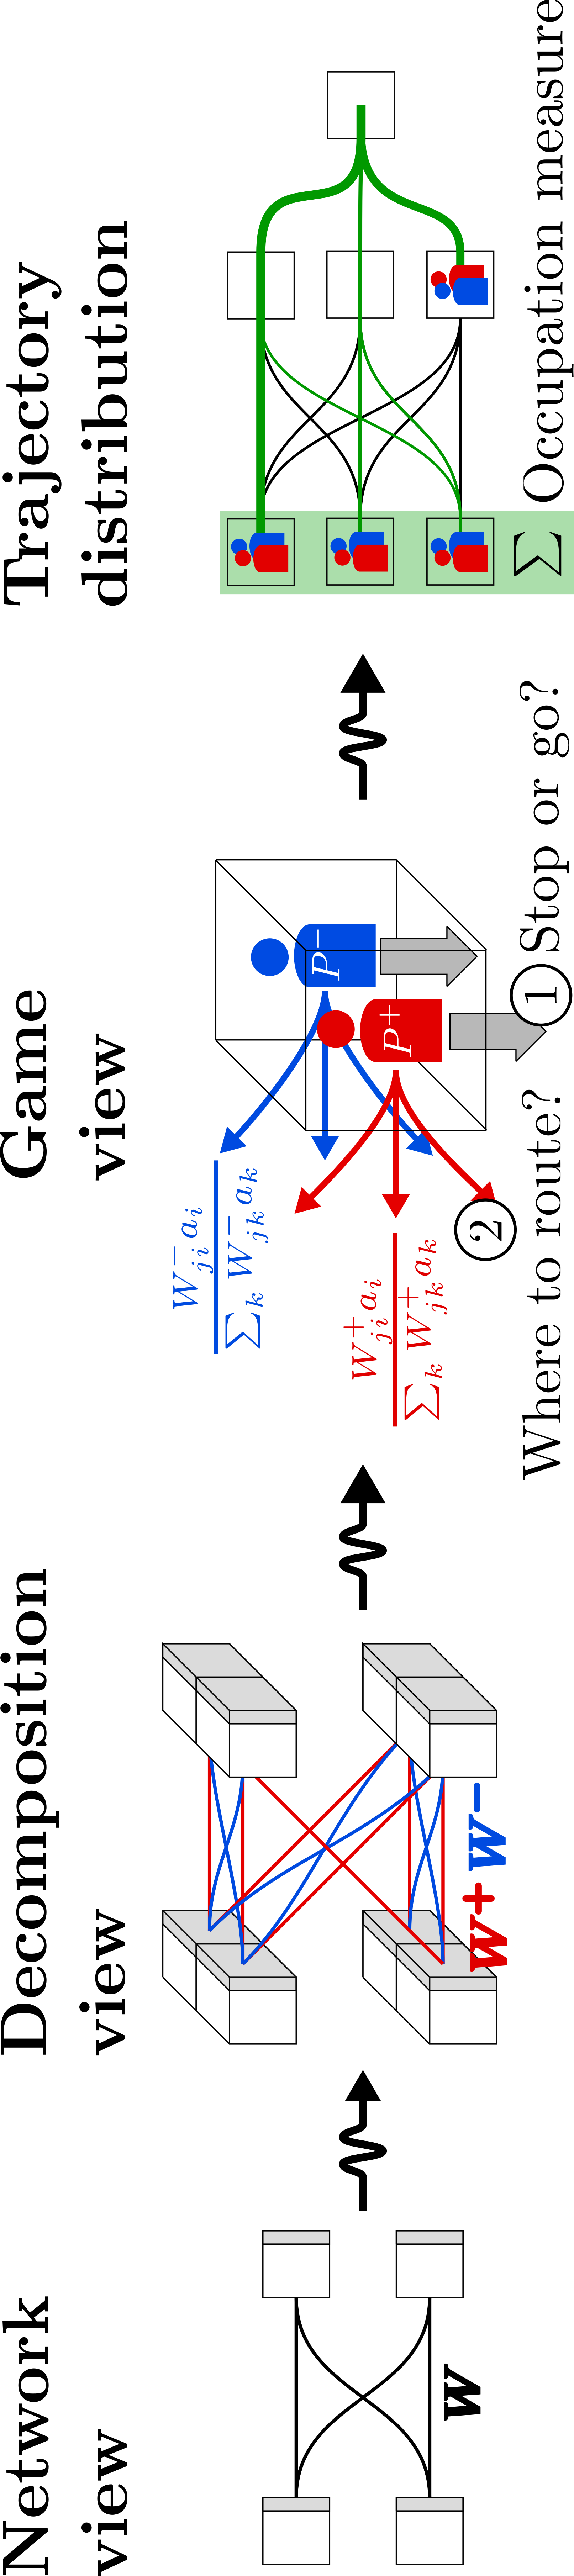
\includegraphics[angle=270,width=0.86\textwidth]
        {figures/ptnb_v2/main_figure.png}
    \caption[The backward pass as a two-player game]{The backward pass as a two-player game. The Stopping Decomposition splits every weight by
    sign, $W = W^+ - W^-$; at each state of the extended graph the players decide (1) stop or continue
    and (2) where to route. Their equilibrium policies induce a distribution over backward
    trajectories, and the discounted occupation measure of that distribution at the input states is the
    attribution map.}
    \label{fig:game_trajectory_overview}
\end{figure}

The two parts are related, but the games are not reformulations of the split methods. The \ac{dc} decomposition supplies the convex, monotone streams on which split-based attribution operates. The Stopping Decomposition shares its sign-split of the weights and gates both streams with the original activations, which exposes the active signed paths on which the \ac{sg} is played. The \ac{rg} is a separate routing construction on this sign-split graph, chosen to recover the stated $\alpha\beta$-\ac{lrp} rule (Section~\ref{sec:related_work_games}). Their shared theme is to make the backward computation explicit.

These representations support complementary ways of developing attribution methods. SplitCAM, SplitLRP, and SplitGrad operate on the DC representation; the game formulation makes stopping decisions, sign switches, and routing policies available for principled modification. Policy regularization, risk aversion, and extended action sets translate desired properties such as focus and stability into explicit changes of backward rules. \begin{changed}Figure~\ref{fig:vit_temperature} illustrates this control: lowering the routing temperature produces sparser heatmaps concentrated on fewer image regions, with the model and input held fixed.\end{changed} Extensions to multiplicative operations and attention carry the framework beyond the basic MLP setting.

\begin{changed}
Together, the two papers establish network decomposition as a basis for improved attribution and a common mathematical account of backward rules. SplitCAM improves localization and Selectivity on pretrained VGG-16 and ResNet-18, while SplitLRP achieves the lowest Maximum Sensitivity in the VGG-16 comparison. The game framework unifies gradients and $\alpha\beta$-\ac{lrp} and turns routing modifications into strong ViT attribution methods: selected RG reaches Attribution Localization $0.711$ against $0.644$ for the best baseline in the original localization-selected benchmark, with the lead transferring to Pascal VOC without retuning. These results demonstrate the practical value of exposing and modifying a model's internal attribution computations (Chapter~\ref{ch:experiments}).
\end{changed}

The trajectory perspective also returns to the concern raised by randomization sanity checks. Attribution maps aggregate signed, discounted contributions from many backward trajectories and need not reveal how those trajectories traverse the model. Hellinger diagnostics compare the normalized routing laws themselves, complementing comparisons of the resulting maps. We demonstrate that cascading parameter randomization changes trajectory distributions from the first randomized layer, even when attribution maps retain substantial structure. Across VGG-16, ResNet-50, and ViT-B/16, mean trajectory distance increases with input noise. Pairwise comparisons using the unconditioned distance show larger mean distances between classes than within classes, and still larger distances between natural images and Gaussian noise, for the Stopping Game on VGG-16 and the Routing Game on ResNet-50 and ViT-B/16 (Chapter~\ref{ch:trajectory}).

The thesis answers its three research questions as follows. \emph{What structure can be exposed without changing the network's function?} The framework separates contributions into monotone convex streams and groups network paths by the sign of the product of weights along each path. \emph{What does a backward attribution actually calculate?} Derivative identities and game occupation measures relate local propagation rules to explicit global objects. \emph{How can these representations guide the design and evaluation of attribution methods for visual inspection?} Stable implementations, principled modifications of backward rules, and complementary map- and trajectory-level diagnostics provide a novel basis for assessing what an attribution reveals and where its limitations lie.

\paragraph{Publication basis.}
This thesis brings together and extends two research works on which the thesis author is first author:
\begin{itemize}
\item \emph{Hidden Monotonicity: Explaining Deep Neural Networks via their DC Decomposition}, coauthored with Georg Loho, was published at \textbf{CVPR 2026 and selected as a Highlight}~\parencite{hiddenMono}.\footnote{Official CVPR listing: \url{https://cvpr.thecvf.com/virtual/2026/poster/36564}.}

\item \emph{Playing the Network Backward: A Game-Theoretic Attribution Framework}, coauthored with Jim Berend, Georg Loho, Sebastian Lapuschkin, and Wojciech Samek, is a \textbf{preprint}~\parencite{playingBackward2026}.
\end{itemize}
Beyond the two papers, the thesis adds exact DC decompositions for smooth activations (GELU, Swish, sigmoid, and softplus), softmax, and LayerNorm, and combines them into a constructive Transformer decomposition for arbitrary finite depth. It connects the papers' decomposition and game frameworks, adds a partial Lean formalization, and reuses their experimental outputs. Appendix~\ref{app:publication_provenance} records publication provenance and tool use.

\paragraph{Author's contribution.}
My principal contributions to the two underlying papers were developing the theory, developing and conducting the experiments, and writing all appendices and most of the paper text outside the introductions. These contributions were developed in collaboration with the coauthors listed above. Section~\ref{app:author_contribution} distinguishes my contributions to the papers from the subsequent thesis integration and formalization.

\section{Contributions of This Thesis}\label{sec:contributions}

The thesis makes six contributions.

\begin{enumerate}
    \item \textbf{A general framework of network decompositions.}
    We place DC, stopping, mixing, and regularized decompositions in a common framework and extend the DC construction to smooth activations, including GELU, Swish, sigmoid, and softplus.

    \item \textbf{\acs{dc} decompositions for \acs{relu} networks, \acsp{cnn}, and Transformers.}
    We stabilize the split forward and backward passes of pretrained ReLU networks and CNNs without changing their predictions. We also give a first explicit exact DC decomposition algorithm for the deterministic Transformers defined in Section~\ref{sec:transformer_dc}, addressing the extension left open in \emph{Hidden Monotonicity} through splits of softmax, LayerNorm, and non-piecewise-linear GELU.

    \item \textbf{A game-theoretic account of backward attribution.}
    We represent gradients and $\alpha\beta$-\ac{lrp} through two-player games, providing a common basis for comparing and modifying their propagation rules and diagnosing changes in backward routing.

    \item \textbf{New attribution methods with improved faithfulness and localization.}
    Using the \acs{dc} decomposition, we develop SplitCAM, SplitLRP, and SplitGrad; SplitCAM improves Selectivity and localization on VGG-16 and ResNet-18. Game-derived attribution leads the original ViT-B/16 benchmark in Attribution Localization on ImageNet-S~\parencite{gao2022luss}; additional controls examine its trade-offs with faithfulness and robustness.

    \item \textbf{Directly trained difference models.}
    We train differences of convex or monotone networks and inspect their stream gradients on MNIST, as a counterpart to decomposing pretrained models.

    \item \textbf{Trajectory distributions and Hellinger diagnostics.}
    We represent backward calculations as trajectory distributions and use the known geometric-mean factorization of \textcite{Kazakos1978} to compute Hellinger comparisons. We develop terminal-state and survival-conditioned diagnostics and apply trajectory comparisons to parameter randomization, revealing routing changes that attribution maps can obscure (Chapter~\ref{ch:trajectory}).
\end{enumerate}

Table~\ref{tab:guarantee_map} maps each object studied in the thesis to its established result, the supporting evidence, and the scope of that statement.

\begin{table}[htbp]
\TableContent{
\centering
\small
\setlength{\tabcolsep}{4pt}
\begin{tabularx}{\linewidth}{@{}>{\raggedright\arraybackslash}p{0.17\linewidth}>{\raggedright\arraybackslash}X>{\raggedright\arraybackslash}p{0.2\linewidth}>{\raggedright\arraybackslash}p{0.29\linewidth}@{}}
\toprule
Object & Established result & Evidence & Scope \\
\midrule
Exact \acs{dc} streams & Recovery of the network function; convex, coordinatewise non-decreasing streams on the doubled inputs & Chapters~\ref{ch:decompositions} and~\ref{ch:transformers} & Mathematical property of the streams; their roles are defined by the decomposition. \\
Stabilized split passes & Forward and backward invariants of the shifted and scaled passes & Section~\ref{sec:stabilization_dc}; split-method experiments in Chapter~\ref{ch:experiments} & Recovery of the stream difference; convexity and monotonicity are stated for the exact streams. \\
Transformer \acs{dc} implementation & Reconstruction of outputs and gradients to machine precision & Section~\ref{app:transformer_dc_numeric} & Nine float64 runs on pretrained ViT-B/16. \\
Conditioned ViT SplitCAM & Attribution results with fixed attention and LayerNorm & Section~\ref{sec:vit-extension} & Exploratory comparison of complete attribution pipelines. \\
\acs{sg} and \acs{rg} anchors & Recovery of gradients and of the stated $\alpha\beta$-\acs{lrp} rule & Chapter~\ref{ch:game_theory}; Sections~\ref{app:rebuttal-sg} and~\ref{app:rebuttal-rg} & Stated propagation conventions; benchmark readouts and deformed modes are specified separately. \\
Hellinger diagnostics & Exact comparison of the specified routing laws & Section~\ref{sec:probabilistic_foundations}; Chapter~\ref{ch:trajectory} & Routing probabilities of the diagnostic processes, which omit the bias action for the \acs{rg}; discounts are not part of the compared law. \\
\bottomrule
\end{tabularx}
}%
\caption[Map of guarantees and evidence]{Map of guarantees and evidence: what is established for each object of the thesis, where the evidence is, and the scope of the statement.}
\label{tab:guarantee_map}
\end{table}

\section{Positioning within the Literature}\label{sec:related_work}

This brief section positions the thesis along its three research questions; additional chapter-opening discussions cover related work regarding games and propagation rules (Section~\ref{sec:related_work_games}) and Transformer interpretability (Section~\ref{sec:related_work_transformers}).

\subsection{What Structure Is Hidden Inside a Trained Network?}
The use of monotonicity and convexity to structure interpretable models runs from monotonic networks \parencite{Sill1997_MonotonicNetworks,Daniels2010_MonotoneNN} through certified and lattice-based monotone models \parencite{Liu2020CertifiedMonotone,Gupta2016MonotoneLattice,Sivaraman2020_COMET,Nguyen2023_MonoNet,Runje_2023} to \acp{icnn} \parencite{Amos2017} and convex network calculus \parencite{Bach2017ConvexNN,Calafiore2019DLSE,sivaprasad2021curious}. \ac{dc} decompositions bridge this to unconstrained networks: classical \ac{dc} programming \parencite{Tao1997_DCProgramming,LeThi2018DCA,Sriperumbudur2009CCCP} studies optimization with such decompositions, while the representation theory of piecewise-linear functions as differences of convex ones \parencite{Melzer1986_PLasDC,Kripfganz1987_PWAasDC,Zalgaller2000_DCRepresentation,Griewank2020_PolyhedralDCDecomposition,Schlueter2021_ConvexDecompPAF,Koutschan2024_MinimalArity,Kazda2024_LP_DCPLA,Brandenburg2025_DecompositionPolyhedra} guarantees the split exists; \textcite{Awasthi2023DCNN} and \textcite{Siahkamari2020_DCRegression} construct essentially the split used here, for optimization and regression, and CDiNN-type architectures make the difference structure trainable \parencite{Sankaranarayanan2021CDINN,Chen2025_RCDiNN}. This thesis studies the split's numerical instability in deep networks and its use for explanation. The geometric reading rests on the identification of \ac{relu} networks with \ac{cpwl} maps \parencite{Arora2018,BalestrieroBaraniuk2018MadMax,huchette2025deeplearningmeetspolyhedral} and their tropical representations \parencite{Zhang2018}.

\subsection{Visual Attribution Methods and Their Interpretation}\label{subsec:visual_attribution_related}
A heatmap visualizes scores assigned to pixels or spatial features for a chosen prediction. The scores may describe sensitivity, differences from a reference, or redistributed relevance. White-box methods access model weights, activations or derivatives. Our split and game methods use this access to study the network representation and its backward rules.

Gradient saliency measures local class-score sensitivity~\parencite{Simonyan2014}; SmoothGrad averages gradients over noisy inputs~\parencite{Smilkov2017}. Deconvolution and guided backpropagation modify backward activation gates~\parencite{ZeilerFergus2014,Springenberg2015}, while PatternAttribution uses signal directions learned from data~\parencite{Kindermans2018PatternAttribution}. SplitGrad reads stabilized split-stream sensitivities (Section~\ref{sec:split_grad}); the stopping game represents ordinary gradients through discounted occupation measures, exposing their backward routing (Chapter~\ref{ch:game_theory}).

Integrated Gradients integrates gradients along a path from a reference input~\parencite{Sundararajan2017}; DeepLIFT propagates activation differences relative to reference activations~\parencite{Shrikumar2017}. Both explain $f(x)-f(x_0)$ relative to a baseline $x_0$. DeepLIFT's RevealCancel rule separates positive and negative activation changes, averaging each group's effect with and without the other group present. We can read this as a debate over the change from the reference, retaining opposing effects that may cancel in their total. Our DC split makes opposition explicit in the forward function $f=g-h$, without requiring a reference image. RevealCancel uses local cooperative Shapley allocations; our zero-sum games describe backward routing through player policies.

CAM assumes a specific classifier architecture: global average pooling of the final convolutional feature maps followed by a linear class readout. The classifier's weights combine those maps into a class-specific heatmap~\parencite{Zhou2016}. Grad-CAM, LayerCAM and HiResCAM instead obtain weights from derivatives of the class score $f_c$. Let $A^k_{ij}$ be the activation in channel $k$ at spatial position $(i,j)$, $G^k_{ij}:=\partial f_c/\partial A^k_{ij}$ its gradient, $N$ the number of spatial positions, and $[t]_+:=\max\{t,0\}$. All three sum weighted activations across channels, $S_{ij}=\sum_k w^k_{ij}A^k_{ij}$, with
\[
 w^k_{ij}=\begin{cases}
 \displaystyle\bar G^k:=\frac{1}{N}\sum_{u,v}G^k_{uv}
   & \text{Grad-CAM: one average gradient per channel},\\[1mm]
 [G^k_{ij}]_+ & \text{LayerCAM: each local gradient, clipped at zero},\\[1mm]
 G^k_{ij} & \text{HiResCAM: each local gradient, including its sign}.
 \end{cases}
\]
Grad-CAM uses the same weight at every position in a channel~\parencite{Selvaraju2017}. Guided Grad-CAM multiplies its upsampled map pointwise by the Guided Backpropagation map. LayerCAM discards negative gradients before multiplication~\parencite{Jiang2021LayerCAM}; HiResCAM retains them, allowing signed products to cancel across channels~\parencite{Draelos2020hirescam}. Grad-CAM and LayerCAM then display $[S_{ij}]_+$; HiResCAM's defining map is $S$, which can likewise be clipped for positive-only visualization. This final clipping differs from LayerCAM's clipping before summation. Grad-CAM++ also uses channel weights, obtained by weighting positive gradients before pooling~\parencite{Chattopadhay2018}. SplitCAM uses local products of decomposed activations and shifted split-stream sensitivities (Section~\ref{sec:split_cam}), omitting both positive-gradient filtering and final map clipping.

\paragraph{LRP rules.}\label{par:lrp_rules}
LRP redistributes the prediction through weights and activations~\parencite{Bach2015,Montavon2018}. For a bias-free ReLU layer, let $a_i\ge0$ be its input activations, $w_{ij}$ the weight from neuron $i$ to neuron $j$, and $R_j$ the relevance passed back by an active neuron $j$. The $\varepsilon$- and $\gamma$-rules have the common form~\parencite{Montavon_2022_gammaLRP}
\begin{equation}\label{eq:lrp_gamma_overview}
 R_i=\sum_j\frac{a_i\bigl(w_{ij}+\gamma[w_{ij}]_+\bigr)}
 {\varepsilon+\sum_k a_k\bigl(w_{kj}+\gamma[w_{kj}]_+\bigr)}R_j,
 \qquad \varepsilon,\gamma\ge0.
\end{equation}
With $\varepsilon=\gamma=0$, this is the basic $z$-rule. The $\varepsilon$-rule ($\gamma=0$) enlarges small denominators, absorbing some relevance. The $\gamma$-rule ($\varepsilon=0$) multiplies positive contributions by $1+\gamma$ before renormalization, reducing cancellation with negative contributions. The $\alpha\beta$-rule instead normalizes positive and negative contributions separately and weights them by $\alpha$ and $-\beta$, with $\alpha,\beta\ge0$ and $\alpha-\beta=1$; $(\alpha,\beta)=(1,0)$ gives the $z^+$-rule. Section~\ref{ptnb:sec:background} specifies its bias and stabilizer conventions. Deep Taylor decomposition derives selected rules through local Taylor expansions~\parencite{Montavon2017DeepTaylor}.

SplitLRP applies relevance propagation to the DC split network, starting from its positive output stream (Section~\ref{sec:split_lrp}). Our routing game gives the full $\alpha\beta$-LRP family a representation through policies and signed discounted occupation measures, providing a common basis for comparison with the gradient-recovering stopping game.

White-box access also supports perturbation-based explanations: Meaningful Perturbation optimizes masks with gradients~\parencite{FongVedaldi2017}, ShearletX optimizes sparse masks in a directional image representation~\parencite{Kolek2023_ShearletX}, and EVA propagates verified output bounds~\parencite{Fel2023_EVA}. Their analysis of input changes complements our study of contributions and backward routing. LIME and KernelSHAP instead use model-agnostic input--output queries~\parencite{Ribeiro2016,LundbergLee2017}; both serve as black-box baselines for the game methods (Appendix~\ref{app:baselines}).

\subsection{Attribution in Language Models}
Attribution can identify specialized attention heads and help test whether a language model draws on supplied context or knowledge acquired during training~\parencite{Kahardipraja2025Atlas,Voita2019}. Attribution patching and related methods test component roles through interventions~\parencite{Syed2024AttributionPatching,Kramar2024AtPStar,Hanna2024Faithfulness}. Other work studies oversight and intervention. \textcite{Gurnee2026Workspace} investigate \emph{J-space}, representations accessible to verbal report, and find evidence for a \emph{global workspace} shared across internal computations. Their gradient-based Jacobian lens (J-lens) surfaces evaluation-awareness signals; in a model trained to conceal an objective of pleasing reward-model preferences, it revealed readouts containing ``reward'' and ``bias'' even on ordinary prompts. The R-lens of \textcite{Blank2026RLens} replaces gradient transport with LRP rules and recovers intermediate variables more reliably in early layers; ablations support greater causal relevance of its readout directions on multihop questions. Attribution can also guide decoding toward supplied instructions or evidence~\parencite{Komorowski2026AGD}: under matched settings, AttnLRP yielded stronger instruction adherence than Input$\times$Gradient across three tested models, alongside lower output-quality scores. \textcite{Biton2026HiddenRequest} use LRP-guided decoding to increase ethical responses to unethical requests by emphasizing tokens expressing the harmful act. These studies complement our focus on the mathematical structure of backward rules in Transformers.

\subsection{What Connects Different Backward Attribution Rules?}
The ReLU Net Game of \textcite{Gaubert2025} represents forward evaluation as the value of a zero-sum stopping game. We use the stopping decomposition to connect this game representation to backward attribution. Two related approaches describe how attribution flows through a network: Excitation Backprop represents the $(\alpha,\beta)=(1,0)$ rule of \ac{lrp} as an absorbing Markov chain for non-negative activations, omitting biases and stabilization~\parencite{Zhang2018pointinggame}. The \ac{nrm} framework assigns signed relevance measures to neuron walks~\parencite{Xiong2026nrm}. Our stopping game adds an opponent to the probabilistic view. KernelSHAP~\parencite{LundbergLee2017} uses a cooperative game over input coalitions, rather than a game on the network's computational graph.

The game formulation also provides a basis for modifying backward rules. The softplus-based curvature reduction of \textcite{Dombrowski2020} appears here as entropy regularization of stopping decisions, while risk-sensitive control~\parencite{zhang2021risk} motivates the risk-averse modes. Section~\ref{sec:related_work_games} develops these connections.

For Transformers, related approaches include attention rollout and flow~\parencite{Abnar2020attention}, relevance propagation~\parencite{Chefer2021ICCV,Chefer2021GenericAttention,Ali2022AttnLRP,Achtibat2024AttnLRP}, and methods addressing attention artifacts~\parencite{Wrobel2024,darcet2024vision}. Section~\ref{sec:related_work_transformers} compares these approaches with our treatment of attention and multiplicative operations.

\paragraph{Outline.}
Chapter~\ref{ch:foundations} assembles the foundations: network notation, \ac{cpwl} mappings, convexity and monotonicity, \acp{mdp} and zero-sum games, including the ReLU Net Game of Gaubert and Vlassopoulos, and probability distances for layered Markov processes. Chapter~\ref{ch:decompositions} develops the decomposition framework, numerical stabilization, the \ac{cnn} extension, and SplitCAM, SplitLRP and SplitGrad. Chapter~\ref{ch:game_theory} develops the two-player stopping and routing games and their attribution modes; Chapter~\ref{ch:transformers} extends the framework to multiplicative operations and \acp{vit}. Chapter~\ref{ch:experiments} reports the attribution benchmarks and the directly trained difference-of-convex models on MNIST. Chapter~\ref{ch:trajectory} develops the trajectory-distribution view and its Hellinger diagnostics; Chapter~\ref{ch:conclusion} concludes with future directions.

\paragraph{Reading guide.}
The chapters need not be read linearly. Chapter~\ref{ch:decompositions} requires only the network notation of Section~\ref{sec:nn_notation_pwl} and the convexity and monotonicity notions of Section~\ref{sec:convex_monotone_foundations}. Chapter~\ref{ch:game_theory} builds on the game-theoretic foundations of Section~\ref{sec:game_theory_mdp_foundations} and, within Chapter~\ref{ch:decompositions}, on the Stopping and regularized decompositions (Sections~\ref{sec:stopping_decomposition} and~\ref{sec:regularized_decompositions}). In Chapter~\ref{ch:transformers}, the Transformer decomposition (Sections~\ref{sec:multiplicative_splits} and~\ref{sec:transformer_dc}) continues Chapter~\ref{ch:decompositions}, while the attention game (Section~\ref{sec:attention_routing_game}) continues the Routing Game of Section~\ref{ptnb:sec:routing}. The probability distances of Section~\ref{sec:probabilistic_foundations} are used only in Chapter~\ref{ch:trajectory} and can be deferred until then. Readers interested mainly in the empirical results can proceed to Chapter~\ref{ch:experiments} after the split-based attribution methods of Section~\ref{sec:split_attribution_concept} and the game modes of Section~\ref{ptnb:sec:modes}.
